\newpage
\section{SYSTEM DESIGN}

\subsection{System Overview}
The system uses initially predicts the personality of the user with the help of their social media account(facebook). Thus initially a classifier is to be trained to classify the personality of the user on the basis of their status update. Afterwards, the predicted personality of the user is to be used as one the metrics for the similar user computation in collaborative filtering and the effect of the personality on the collaborative filtering engine was observed.

\subsection{System Architecture}
The give figure below is the architectural diagram of the project showing the process that are involved during the development of the project.

\begin{figure}[!ht]
\centering
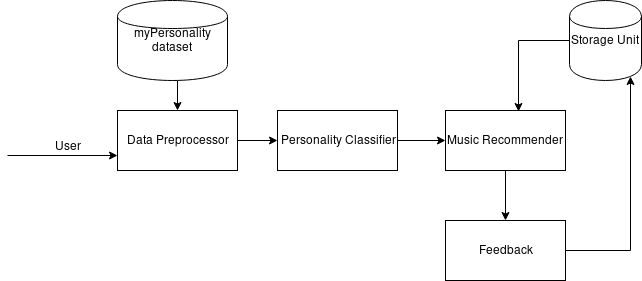
\includegraphics[width = 16 cm]{fig/system.png}
\caption{block diagram of the system}
\label{fig:project}
\end{figure}

\begin{itemize}
	\item Data Preprocessor: This subsystem is responsible for the conversion of the status update of the user from the dataset \cite{dataset} as well user logged in via API \cite{api} into vector representation via the use of bag of word and tf-idf model.\\
It is responsible for:
		\begin{enumerate}
			\item Lower casing the status update.
			\item Tokenization
			\item Filtering stop words
			\item Filtering parts of speech
			\item Stemming
			\item Conversion of textual data to vector representation(numerical form)
		\end{enumerate}
	\item Classifier: After the vector representation of the status update,this subsystem is responsible for personality prediction. Classifier are trained by the admin in the system using the dataset \cite{dataset} in order to predict a personality. In the project there are three classifier model used for the personality classification.\\
They are:
\begin{enumerate}
	\item Naive Bayes Classifier
	\item Logistic Regression
	\item KNN 
\end{enumerate}
\item Recommender System: The system comprises of the eight models for the recommendation of the music to the user.\\
They are:
\begin{enumerate}
	\item Global Baseline Approach
	\item User to User collaborative filtering with rating matrix
	\item User to User collaborative filtering with personality matrix
	\item User to User collaborative filtering with weighted average of rating and personality matrix
	\item Combination of global baseline and CF with rating matrix
	\item Combination of global baseline and CF with personality matrix
	\item Combination of global baseline and CF with weighted average of rating and personality matrix
	\item Matrix Factorization
\end{enumerate}
\item Storage Unit: It is responsible for storing of user data, music data, user-music-rating data and user-music-recommendation data made by the recommender system. SQLite database is used as the storage unit for the project.
\end{itemize}

\newpage
\subsection{Use Case Diagram}
The use case diagram of the system depicting the actors and their interaction to the system is given in the figure below:
\begin{figure}[!ht]
\centering
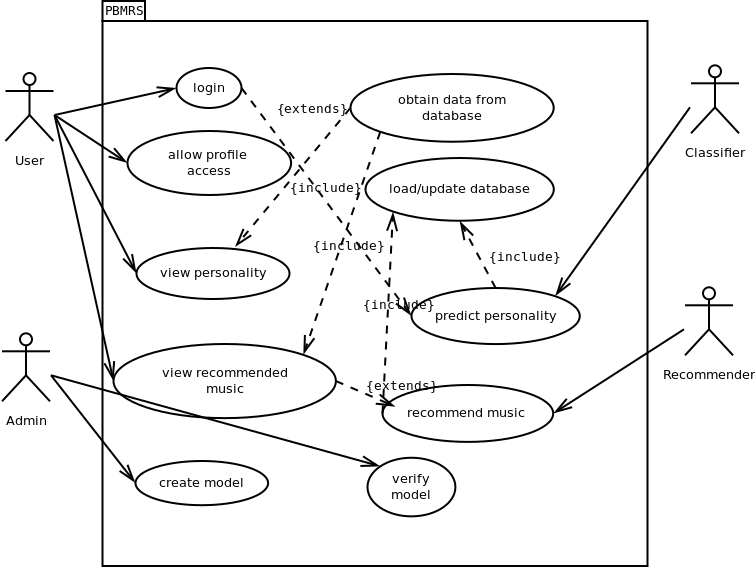
\includegraphics[width = 16 cm]{fig/usecase.png}
\caption{Use Case Diagram of the System}
\label{fig:usecase}
\end{figure}

From the above diagram, it is clear that the system consists of four actors.They are:
\begin{itemize}
\item User: They are the ones who will be using the system directly. The users will be able to do the actions like login, viewing recommendation and listening to a music. 
\item Admin: Admin is directly responsible for training a classifier subsystem and recommender subsystem, creation of model for the storage engine and verification of all of these subsystem.
\item Classifier: It is responsible for the classification of the personality of the user and update of the database.
\item Recommender: It is responsible for the recommendation of the music to the user and also update of the database.
%\item Storage Handler: It is responsible for the creation of the data base model and storage of system data.
\end{itemize}

\newpage
\subsection{ER Diagram}
The  ER diagram depicting the entities used in the system and relationship between them is given below:
\begin{figure}[!ht]
\centering
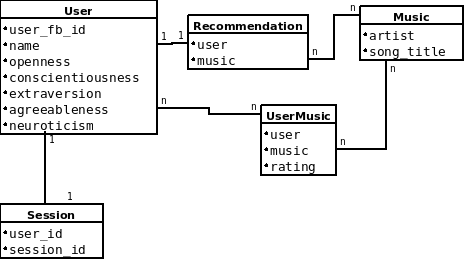
\includegraphics[width = 15 cm]{fig/er.png}
\caption{ER diagram of the System}
\label{fig:er}
\end{figure}
The entities in the system are:
\begin{enumerate}
	\item Session: It consists of attributes: session id and user id and has one to one relationship with user.
	\item Music: It consists of attributes: artist and song title and also has  many to many relationship with the user-music and recommendation. 
	\item User: It consists of attributes user id, name and personality traits attributes and has  many to  many relationship with user-music and one to one with the session with session and recommendation. 
	\item Recommendation: It consists of attributes user and music and has one to one relationship with user while many to many relationship with music.
	
	\item User-Music: It consists of attributes user, music and rating and many to many relationship with user and music. 
\end{enumerate}
\newpage
\subsection{Activity Diagram}
\begin{figure}[!ht]
\centering
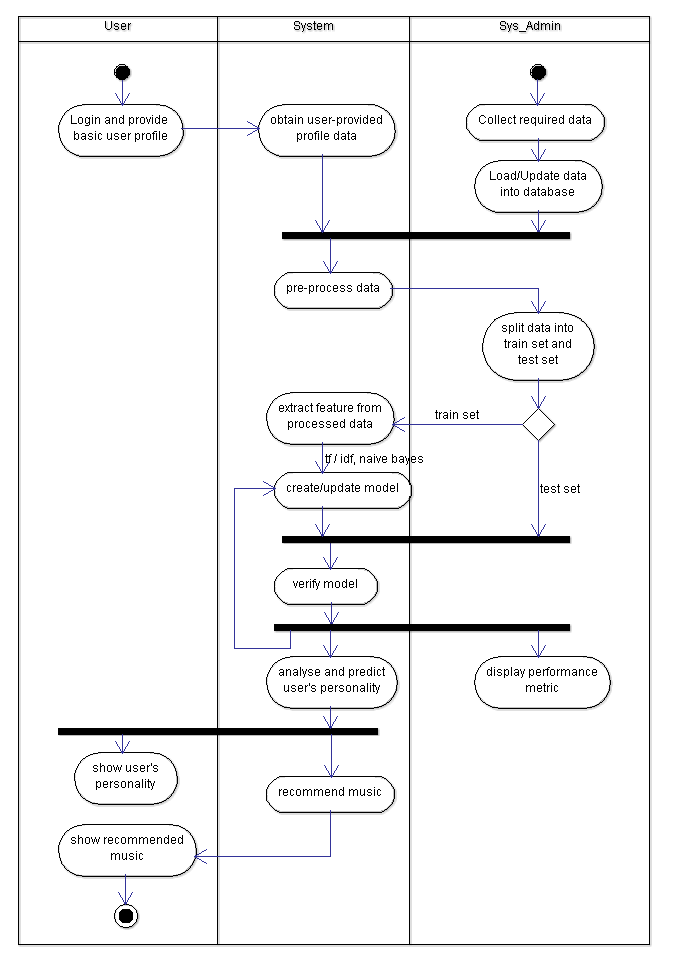
\includegraphics[width = 12 cm]{fig/Activity.png}
\caption{Activity Diagram of the System}
\label{fig:activity}
\end{figure}
The diagram above shows the activity digram of the system. It depicts how the user, admin and system interacts with each other. Initially user login into the system providing the basic user profile information. Afterwards, the status of the new/old user is used to predict the personality with classifier. Then music is recommended to user. Besides, the user can also view his personality.

\newpage
\subsection{Data Flow Diagram}
The figure given below is the data flow diagram of the project showing the flow of data within the system. 

\begin{figure}[!ht]
\centering
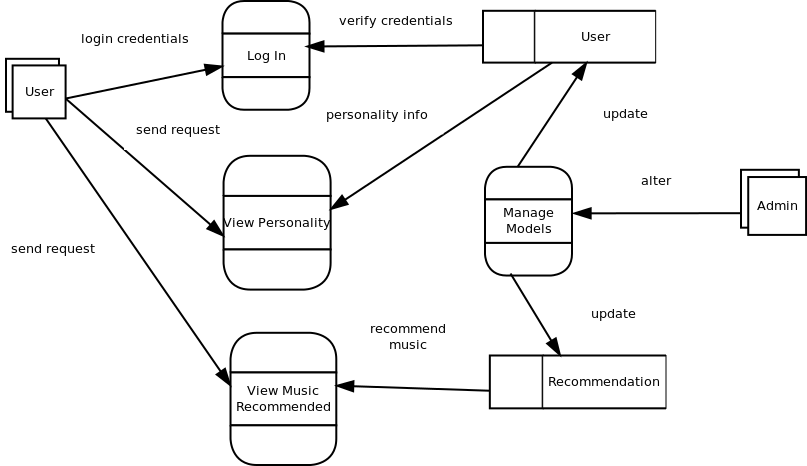
\includegraphics[width = 16 cm]{fig/dfd.png}
\caption{Data Flow Diagram of the System}
\label{fig:dfd}
\end{figure}

It is the level-1 dfd, with the two entities User and Admin. User is responsible for log in, view personality and view recommended music, all of which takes data from the user and recommendation store, to provide a data to the user. Besides admin is responsible for creating and altering models(classifier,recommender,database) all of which are reflected within the user and recommendation store.
\newpage
\subsection{Front End of the System(User Interface)}
User Interface is one of the major part of the system. It is where a user will login through their Facebook id in order to experience the personalized based music listening. User is able to able to view his personality via the website and also view the detailed description about the personality traits. Personality classification and music recommendation are all performed in the backend of the system. 

% Following are the snapshots of our system UI:
% \begin{figure}[!ht]
% \centering
% 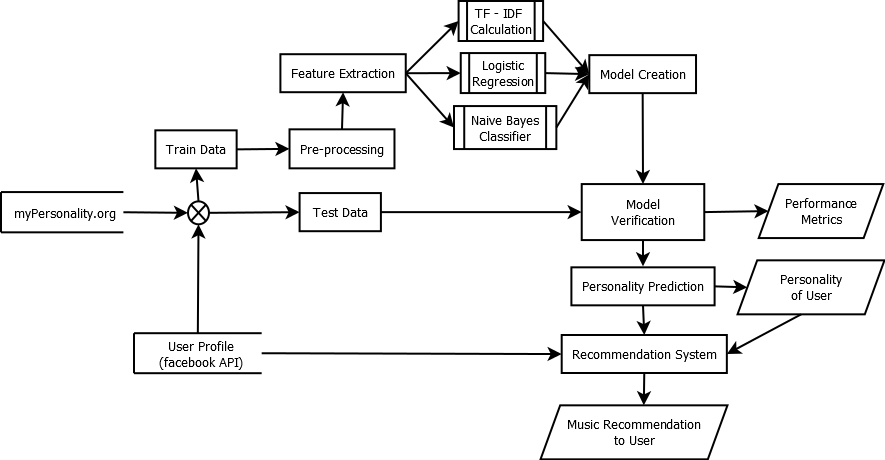
\includegraphics[width = 16 cm]{fig/System.png}
% \caption{Front of the System}
% \label{fig:front}
% \end{figure}

% \newpage
\subsection{Back End of the System}
After the user login through Facebook, the user post are extracted through Graph API. The data obtained goes through the preprocessor where it's performs various NLP techniques such as tokenization, POS tagging at the end of which feature vector is given as output by this subsystem. Thus created vector is passed through the classifier, that classifies the personality of the user, which is then stored in the database and is also fed into user-to-user collaborative filtering engine to determine the similar user and recommend the music to the user.Besides there are also other recommendation model, one with the least RMSE value is used for the recommendation of the music. Thus obtained result is sent back to the front end and is displayed to the user. Then the user can view recommended music and his/her personality traits too.
